\chapter{The $\alpha$-shapes approach to compute the boundaries in target phase space}\label{chap:boundaries_alpha}
In the previous chapter we presented a new ray tracing approach based on PS. We explained that, in order to compute the target photometric variable, it is useful to know the boundaries of the regions with positive luminance in target PS. Ray tracing in PS allows tracing only the rays close to these boundaries. 
In order to detect the shape formed by those rays an $\alpha$-shapes approach is employed, \cite{portegies2013fast}. 
The $\alpha$-shapes methods are widely used to reconstruct an unknown surface from a set of data points, \cite{guo1997surface}. 
It can be very hard to select the suitable value of the parameter $\alpha$ and, in most cases it can be selected only by numerical simulations.
We develop a technique based on $\alpha$-shape that gives a criterion to determine the value of the parameter $\alpha$ for which the better approximation of the boundaries is obtained.  An overview of the state of art about $\alpha$-shapes methods is provided in Section \ref{sec:alpha-shapes}; the technique used for computing the $\alpha$ value is explained in Section \ref{sec:Tir_alpha}; the results for two different kind of total internal reflection (TIR) collimator are given in last paragraph of this chapter.
\section{The $\alpha$-shapes approach}\label{sec:alpha-shapes}
Given a finite set $V$ of points, $\alpha$-shapes are geometrical objects that give us an approximation of the shape\footnote{It will become clear through this chapter what we intend with the word \textit{shape}.} formed by the points in $V$.\\ \indent
Before giving a formal definition, we explain an intuitive and nice interpretation of $\alpha$-shapes, \cite{lucieer2004alpha}. 
Let us think to a mass of a stracciatella ice-cream\footnote{Stracciatella ice cream is made with milk-based ice-cream and fine peaces of chocolate, \cite{Wiki3}.}. If we desire to know the shape formed by the chocolate pieces we can start eating the ice cream using a spoon with a spherical shape and trying to do not remove any piece of chocolate. 
We will obtain a shape formed by arcs and points (see Figure \ref{fig:shape2d} for the two-dimensional case).
\begin{figure}[htbp]\label{fig:shape2d}
\begin{center}
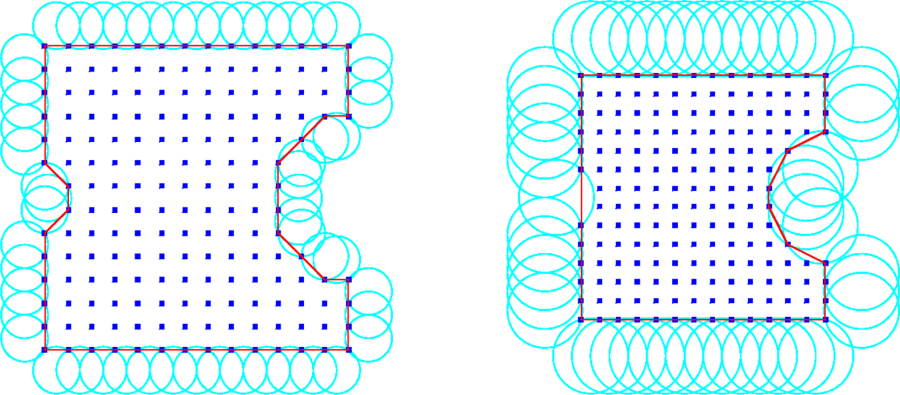
\includegraphics[width=\textwidth]{alpha_shapes2D}
\label{fig:shape}
\caption{Construction of $\alpha$-shape given a set of points (blue dots) in $\mathbb{R}^2$. The boundary of the shape formed by the points cloud (red line) is detected for $\alpha = 1$ (left) and for $\alpha=2$ (right), \cite{sabel2017application}.}
\label{fig:shape2d}
\end{center}
\end{figure}
Straightening the arcs to line segments we obtain broken lines which constitute the boundaries of the so-called $\alpha$-shape formed by the points of the points set $V$. 
A very small spoon will allow us to eat the entire ice cream without eating any piece of chocolate, while with a huge spoon we will not be able to eat any part of the ice cream because at least one chocolate peace will be removed from the ice-cream mass. In this example, the chocolates peaces are the points of $V$ and, the parameter $\alpha$ determines the radius of the carving spoon (the spherical spoon in two-dimension is simply a circle).\\ \indent 
The formal definition of $\alpha$-shape was first given by Edelsbrunner, Kirkpatrick and Seidel in 1983, \cite{edelsbrunner1983shape}. They describe $\alpha$-shape has a generalization of the convex hull of a finite set of point in the plane. Let be $\alpha$ a not negative number $0\leq\alpha<\infty$. 
If $\alpha$ is equal to $0$ the shape degenerates to the point set $V$. On the other hand, when $\alpha\rightarrow\infty$ the $\alpha$-shape is simply the convex hull of $V$. If $0<\alpha<\infty$ the $\alpha$-shape is a polytope of $V$, \cite{edelsbrunner1994three}. The construction of $\alpha$-shape is closely related to Delaunay triangulation of $V$,\cite{mucke1993shapes}. Therefore, a formal definition of triangulations and Delanauy triangulations is now required. \\ \indent
Given a set $V$ of not all aligned points, let us consider the set $E$ of all the straight line segments whose endpoints are in $V$. 
A triangulation $T$ of $V$ is the maximum subset of $E$ such that all the line segments of $T$ intersect only at their endpoints, \cite{lloyd1977triangulations}. \\ \indent 
The Delaunay triangulation $T^{\prime}$ of the points set $V$ has the property (called Delaunay property) that the circle circumscribed by any triangle of $T$ does not contain any point of $V$. A very common used algorithm to construct such triangulation is explained in the following. 
$T^\prime$ is constructed by modifying a general triangulation $T$ such that every point satisfies the Delaunay property. 
Therefore, every triangle (or tetrahedron in three dimensions) that does not satisfy such property is flipped such that the new edge is part of the triangulation, see Figure \ref{fig:Delaunay}. 
More precisely, given an arbitrary triangulation $T$ in two-dimension, for each edge $\overline{ab}$ in $T$ which is not on the boundary of the convex hull the two triangles 
$\Delta_{abc}$ and $\Delta_{abd}$ with the common edge $\overline{ab}$ are found. Then, if either the circumcircle of triangle $\Delta_{abc}$ contains point $d$ or the circumcircle of triangle $\Delta_{abd}$ contains point $c$ the edge $\overline{ab}$ cannot be included in the Delaunay triangulation and, therefore, it is flipped such that the other two possible triangles $\Delta_{acd}$ and $\Delta_{bcd}$ are found. The new edge $\overline{cd}$ locally satisfies the Delaunay property and the triangles $\Delta_{acd}$ and  $\Delta_{bcd}$ are added to the Delaunay triangulation $T^\prime$.  
\begin{figure}[h]\label{fig:Delaunay}
\begin{center}
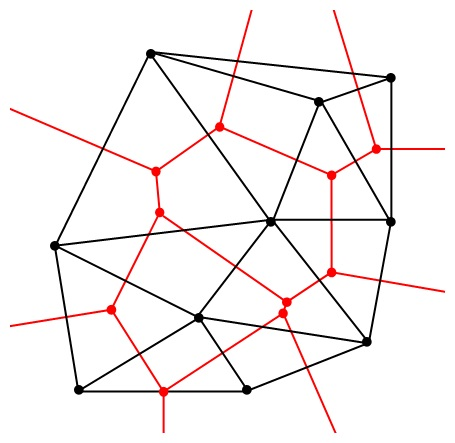
\includegraphics[width=7cm]{Delaunay_Voronoi.jpg}
\label{fig:shape}
\caption{Triangles flipped.}
\label{fig:Delaunay}
\end{center}
\end{figure}
\\ \indent Several others algorithm have been developed to construct a Delaunay triangulation, see for example \cite{lee1980two, renka1997algorithm}.
It can be proved that the Delaunay triangulation $T^\prime$ derived from a triangulation $T$ of a given points set $V$ is unique. It has the property to have the largest minimum angle among all possible triangulation of a point set $V$, \cite{press2007numerical} and, it can be seen as the dual of Voronoi diagram, \cite{fortune1992voronoi}.\\\indent 
Let us consider a finite set of point $V = \{v_1, \cdots, v_N\}\subset \mathbb{R}^2$. For \textit{almost}\footnote{It is needed to specify the word \textit{almost} because some points can have the same distance with two or more points of $V$.} every point $x\in \mathbb{R}^2$, there is a point which is the closest point to $x$. The Voronoi cell of a point $v_\variabile{i}\in V$ contains all points in $\mathbb{R}^2$ which are closer to $v_{\variabile{i}}$., see Figure \ref{fig:Voronoi}. 
The Voronoi diagram of $V\subset \mathbb{R}^2$ is defined as the set of all Voronoi cells, \cite{cazals2005conformal}.  For the definition of Voronoi diagram in higher dimensions see \cite{brown1979voronoi}.
%A formal definition of the Voronoi diagram is given in the following.
%\begin{defn}
%Let $X$ be a metric space with a distance $\textrm{d}$ and $V=\{v_1,\cdots,v_N\}$ a set of point in $X$. The Voronoi cell $V_\variabile{i}$ associated with the point $v_\variabile{i}$ with $v_{\variabile{i}}\in\{1,\cdots,N\}$ is defined as:
%\begin{equation}
%V_\variabile{i}=\{x\in X\; | \;\textrm{d}(x,v_\variabile{i})\leq \textrm{d}(x,v_\variabile{j}) \quad \forall \variabile{j}\neq \variabile{i} \}\,,
%\end{equation}
%The Voronoi diagram is defined as the union $U = \bigcup_{\variabile{i}=1}^N V_\variabile{i}$ where $V_{\variabile{i}}\cap V_{\variabile{j}}= \emptyset$ for $\variabile{i}\neq\variabile{j}$.
%\end{defn}
%Figure \ref{fig:Voronoi}
%\begin{figure}[h]\label{fig:Voronoi}
%\begin{center}
%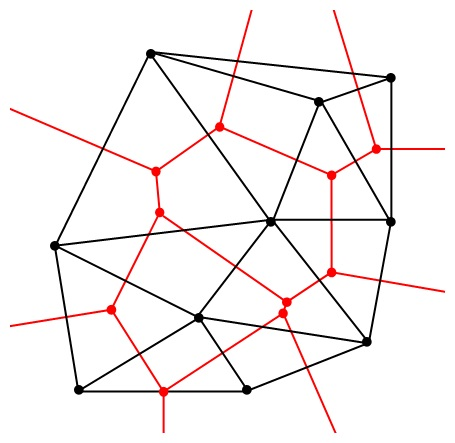
\includegraphics[width=7cm]{Delaunay_Voronoi.jpg}
%\caption{The Delaunay triangulation in black is the dual of the Voronoi diagram in red, \cite{Wiki4}.}
%\label{fig:Voronoi}
%\end{center}
%\end{figure}
Delaunay triangulation triangulates the convex hull of $V$ and, therefore it does not constitutes a suitable method for reconstruct the surface formed by a point cloud. 
\\ \indent An important method in surface reconstruction is the $\alpha$-shapes method, \cite{edelsbrunner2010alpha, guo1997surface}. Starting from the Delaunay triangulation $T^\prime$ of a point set $V$, the corresponding $\alpha$-shape of $V$ is formed by the only triangles of $T^\prime$ that satisfy the so-called "$\alpha$-test".
For each triangle we calculate the radius of the circumcircle. If the radius is larger that $\alpha$ the triangle is removed from the shape. The rule of the parameter $\alpha$ is highly significant in this procedure. We would choose $\alpha$ such the better approximation of the shape formed by the points of $V$ is obtained. 
The choice of the parameter $\alpha$ is closely related to the radius of the circumcircles. A possible strategy is to find the radius of the greater empty circumcircle. Thus $\alpha$ is related to the density $\delta$ of the point sets $V$. In particular $\alpha$ is inversely proportional to $\delta$:
\begin{equation}
\alpha=C\frac{1}{\delta}\;,
\end{equation}
with $C$ a constant and $\delta$:
\begin{equation}
\delta=\frac{N}{\mbox{surface area}}\; ,
\end{equation}
where $N$ is the number of points in $V$ and the surface area is the area inside the boundaries of the region formed by the points cloud. 
For a fixed point set, $\delta$ is given and the value of $C$ needs to be determined by numerical simulations.\\ \indent 
The $\alpha$-shape procedure can be outlined as follows.
\begin{enumerate}
\item Construct a Delaunay triangulation\footnote{In our simulations we use the Matlab function Delaunay.} $T^\prime$ of the point cloud $V$;
\item For every triangles $T^\prime(i)\in T^\prime$ calculates the radius $r(i)$ of the circle circumscribed by its vertices;
\item If $r(i)\leq\alpha$ keep the triangle $T^\prime(i)$ in the triangulation;
\item If $r(i)>\alpha$ remove the triangle from the triangulation;
\item For every triangle return the edges (facets in $3$D) referred to only one triangle (tetrahedron in $3$D), the so-called \textit{free boundary} edges\footnote{In our simulations we use the Matlab function freeBoundary.}.
\end{enumerate}
%% Insert algorithm
%\begin{algorithm}[h]
%\caption{$\alpha$-shape reconstruction}\label{alg:alphashapes}
%\begin{algorithmic}[1]
%\Procedure{$\alpha$-shape}{$V$, $\alpha$}
%\State Construct a Delaunay triangulation of the point cloud $V$
%\State$T^\prime\gets$ all triangles of the Delaunay triangulation
%\State For every 
%\State Calculates the radius of the circle circumscribed by the vertices of every triangle
%\State $r(i) \gets$
%\State For {every triangle in $T^\prime$}
%\State $(\variabile{q}_1^4, \variabile{p}_1^4) \gets \mbox{left and upper corner of source PS: (-\variabile{a}, 1)} $
%\For{$ \variabile{k}= 1 \to 4 $}
%\State Trace the ray with initial coordinates $(\variabile{q}_1^\variabile{k}, \variabile{p}_1^{\variabile{k}})$ in \set{S}{}{};
%\State Calculate the corresponding path $\Pi^{\variabile{k}}$;
%\State $\mbox{Ray}.\variabile{q}\gets [\mbox{Ray}.\variabile{q}, \variabile{q}_1^\variabile{k}]$;
%\State $\mbox{Ray}.\variabile{p}\gets [\mbox{Ray}.\variabile{p}, \variabile{p}_1^\variabile{k}]$;
%\State Store the corresponding path $\Pi^{\variabile{k}}$.
%\State $\mbox{Ray}.\Pi\gets [\mbox{Ray}.\Pi, \Pi^{\variabile{k}}]$;
%\EndFor
%\State VL $\gets [1, 2, 4]$ \Comment{VL = vertices of the left triangle}
%\State VR $\gets [2,3, 4]$   \Comment{VR = vertices of the right triangle}
%\State \Call{Left Triangle}{VL, Ray, $\varepsilon_{\variabile{q}_1}^{\textrm{min}}, \varepsilon_{\variabile{q}_1}^{\textrm{max}}, \varepsilon_{\variabile{p}_1}^{\textrm{min}}, \varepsilon_{\variabile{p}_1}^{\textrm{max}}$}\Comment{Refine the left triangle} 
%\State \Call{Right Triangle}{VR, Ray, $\varepsilon_{\variabile{q}_1}^{\textrm{min}}, \varepsilon_{\variabile{q}_1}^{\textrm{max}}, \varepsilon_{\variabile{p}_1}^{\textrm{min}}, \varepsilon_{\variabile{p}_1}^{\textrm{max}}$} \Comment{Refine the right triangle} \\
%\Return ;
%\EndProcedure
%\end{algorithmic}
%\end{algorithm}
%\\
%Let us define a Voronoi diagram in a metric space.
%The simplest case that we can have is the two-dimensional case that is the case where $X=\mathbb{R}^2$.
%The tuple $\mathcal{S}=\{1,\cdots,n\}\subset \mathbb{R}^2$ is now a set of points. The Voronoi diagram of $\mathcal{S}$ is a subsection of $\mathbb{R}^2$ such that every other region around a point $p\in \mathcal{S}$ contains all points that are closer to $p$ than to every point in $\mathcal{S}$. A triangulation of the point set $\mathcal{S}$ is a set of edges $\mathcal{E}$ whose extremes are points of $\mathcal{S}$ such that the faces of each triangle are bounded by three edges and any edge that is not in $\mathcal{E}$ intersects one of the existing edges. The Delaunay triangulation is the dual graph of the Voronoi diagram: it consists of vertices (the points in $\mathcal{S}$) and it has an edge between two vertices if the two corresponding faces share an edge. \\
\indent Although $\alpha$-shapes are a powerful tool for surfaces reconstruction, there exist surfaces that are not described well by classical $ \alpha $-shapes. Indeed for some surfaces there exist no value of $\alpha$ that includes all desired triangles and deletes all undesired triangles. For example, it can be difficult to obtain a good approximation of a shape formed by a non-uniform points set if the parameter $\alpha$ is determined according to the density of the point cloud. Furthermore, the $\alpha$-shape method does not work well when the shape we need to approximate has a sharp turn or a joint. In this case $\alpha$-shapes often give a "webbed-foot" appearance at such joints since they improperly connect the adjacent surfaces. To overcome this issue, Teichmann and Capps presented alternatives approaches to establish the value of $\alpha$, \cite{teichmann1998surface}. Their anisotropic density-scaled $\alpha$-shapes method constitutes an improvement of  classical $\alpha$-shapes.
\\ \indent There are several ways to determine the value of $\alpha$ \cite{mandal1997selection}; we provide a technique that exploits the conservation of \'{e}tendue in PS. 
%The first step of this method is to make a triangulation of the point cloud.
%Then the key idea is to compute somehow the point-density of each point and use this to get an approximation of the point density of a triangle. In this way one can reduce the $\alpha$-value in areas where the triangle's point density (see equation \ref{delta_t} for the definition) is higher than average in such a way that is possible to obtain a finer level of detail for areas that have an higher density.
%More precisely, each point $ \textbf{p}\in \mathcal{S} $ has a local point density defined as
%\begin{equation}
%\delta (\textbf{p})= \sum_{\textbf{q}\in \mathcal{S}}\Big( 1-\frac{\textrm{d}(q,p)}{\lambda}\Big) \qquad \forall \textbf{q} \mbox{\;\;such that\;\;} \textrm{d}(\textbf{p},\textbf{q})<\lambda\,,
%\end{equation}
%where $ \lambda $ is the constant radius of the local neighborhood and $\textrm{d}(\textbf{x},\textbf{y})$ is the Euclidean distance.
%When local density is larger than the average, that is when
%\begin{equation}
%\delta (\textbf{p}) >\frac{1}{| \mathcal{S} |}\sum_{\textbf{q}\in \mathcal{S}}\delta (\textbf{q})
%\end{equation}
%we know some properties about the region surrounding $\textbf{p}$.
%For instance, if the point set is uniformly distributed then it is possible to find areas with a high-density in the case where there are two closely separated surfaces.  In point sets of non-uniform distribution, high densities are found when the surface presents a joint discontinuity. The algorithm developed by Teichmann and Capps is structured as follow.
%After computing density information for each point they make a triangulation of the point set. Then they calculate the average density  $\delta(t)$ for each triangle $\Delta_{abc}$ defined as:
%\begin{equation}
%\delta(t)=\frac{\delta(a)+\delta(b)+\delta(c)}{3 \mu}\,,
%\label{delta_t}
%\end{equation}
%where $\mu$ is the global average density of the entire point set $\mathcal{S}$.
%If $\delta(t)$ is greater than $1$ the density of the point cloud is higher. Hence is necessary to define another value of $\alpha$:
%\begin{equation}
%\alpha^{\;\prime} = \frac{\alpha}{\delta(t)^\sigma}
%\end{equation} where $\sigma$ is a value that is adjusted by the user.
%If  $\delta$ is less than $1$ the $\alpha$-value is not modified.
%In this way it is possible to have a finer precision on the shape formed by the point set where the density is higher than the average density. Hence it is possible to distinguish two separated objects with different density.
% We want to determine the boundaries in phase space
% Jorg
% It is useful to understand whether the approximation is correct
\section{Determination of $\alpha$ using \'{e}tendue conservation} \label{sec:Tir_alpha}
As mentioned in Section \ref{sec:PSconcept}, in two-dimensions \'{e}tendue can be seen as an area in PS. 
Therefore, given an optical system with a line segment source $\point{S} = [-\variabile{a}, \variabile{a}]$, the \'{e}tendue at the source coincides with the area of \set{S}{}{}, given by:
\begin{equation}\label{eq:etenduesource}
U = 4\n_1 \variabile{a} \sin(\myangle_1^{\textrm{max}})\,,
\end{equation}
 where $\variabile{a}$ is the half length of the source, $\n_1$ the index of refraction of the medium in which the \point{S} is located and $\myangle_1^{\textrm{max}}$ is the maximum value of the angle that the rays make with the normal $\boldsymbol{\nu}_1$ of the source.\\ \indent 
For some optical systems, all the rays emitted by the source arrive to the target, for some others there are also rays that can end up to other detectors. 
Indicating with \set{R}{$1$}{}$(\Pi)$ the regions in source PS formed by the rays that reach the target following path $\Pi$and with \set{R}{}{}$(\Pi)$ the corresponding regions at the target, the \'{e}tendue $U_1$ at source related to the only rays that hit the target is:
\begin{equation}\label{eq:etenduesumsource}
U_1 = \sum_\Pi{U_1\big(\mbox{\set{R}{$1$}{}}(\Pi)\big)},
\end{equation}
where the sum is over all possible paths $\Pi$ and $U_1\big(\mbox{\set{R}{$1$}{}}(\Pi)\big)$ is the contribution to \'{e}tendue given by the rays inside the region 
\set{R}{$1$}{}$(\Pi)$ in source PS given by:
\begin{equation}\label{eq:etendueintegralsource}
U_1\big(\mbox{\set{R}{$1$}{}}(\Pi)\big) = {\int\!\!\int}_{\emph{R}_1(\Pi)} \textrm{d}\variabile{q}\,\textrm{d}\variabile{p}.
\end{equation}
Similarly the \'{e}tendue at the target of the rays emitted by the source is:
\begin{equation}
U_\textrm{t}= \sum_\Pi{U_\textrm{t}\big(\mbox{\set{R}{}{}}(\Pi)\big)},
\end{equation}
with
\begin{equation}\label{eq:etendueintegraltarget}
U_\textrm{t}\big(\mbox{\set{R}{}{}}(\Pi)\big) = {\int\!\!\int}_{\emph{R}(\Pi)} \textrm{d}\variabile{q}\,\textrm{d}\variabile{p}.
\end{equation}
In order to determine the value of $\alpha$ in the $\alpha$-shape procedure that better approximates the boundaries $\partial$\set{R}{}{}$(\Pi)$ we use \'{e}tendue conservation, i.e. $U_{\textrm{t}}= U_1$ as explained in the following.\\ \indent
The $\alpha$-shapes method is applied to every region \set{R}{}{}$(\Pi)$ for a range of values of $\alpha$;
   for each value an approximation of the boundaries $\partial$\set{R}{}{}$(\Pi)$ is obtained and
   the intersection points $\variabile{q}^{\textrm{\,max}}(\Pi,\variabile{p})$ and $\variabile{q}^{\textrm{\,min}}(\Pi,\variabile{p})$ between $\partial$\set{R}{}{}$(\Pi)$
and the horizontal lines $\variabile{p}=const$, with $\variabile{p}\in[-1,1]$, are computed for every path $\Pi$.
Therefore Equation (\ref{eq:etendueintegraltarget}) becomes:
\begin{equation}\label{eq:etenduetarg}
 U_\textrm{t}\big(\mbox{\set{R}{}{}}(\Pi)\big)= \int_{-1}^{1}{\Big(\variabile{q}^{\textrm{\,max}}(\Pi,\variabile{p})-\variabile{q}^{\textrm{\,min}}(\Pi,\variabile{p})\Big)} \textrm{d}\variabile{q}\,\textrm{d}\variabile{p}.
\end{equation} In case more than two intersection points between line $\variabile{p}=const$ and $\partial$\set{R}{}{}$(\Pi)$ occur, the previous equation needs to be generalized. Suppose that $\variabile{r}$ intersection points $\big(\variabile{q}^{\,\variabile{i}}(\Pi,\variabile{p}), \variabile{p}\big)_{\variabile{i} = 1, \cdots, \variabile{r}}$ are found. 
First their $\variabile{q}$ coordinates are ordered in ascending order, second the target \'{e}tendue is calculated using
\begin{equation}\label{eq:etenduetarg1}
 U_\textrm{t}\big(\mbox{\set{R}{}{}}(\Pi)\big) = \int_{-1}^{1}\sum_{\variabile{i} = 1}^{\variabile{m}}
{(\variabile{q}^{\,2\variabile{i}}(\Pi,\variabile{p})}-{\variabile{q}^{\,2\variabile{i}-1} (\Pi, \variabile{p}) )} \textrm{d}\variabile{q}\,\textrm{d}\variabile{p}\,,
\end{equation}
where $\variabile{m}$ is the integer part of $\variabile{r}/2$ with $\variabile{r}$. 
The integrals in Equations (\ref{eq:etenduetarg}) and (\ref{eq:etenduetarg1}) are calculated discretizing the interval $[-1, 1]$
   into $\nbin=100$ sub-intervals of equal length, the so-called bins, and using the trapezoidal rule to approximate the integral.
\\ \indent Matching the value of the \'{e}tendue at the source $U_1$ with the value of the \'{e}tendue at the target $U_{\textrm{t}}$, a unique value $\alpha_{c}$ of $\alpha$  is determined. Implemented the $\alpha$-shapes procedure with $\alpha = \alpha_c$, the best approximation of the boundaries $\partial$\set{R}{}{}$(\Pi)$ is found and the intensity at the target can be calculated.\\ \indent If two intersection points between $\variabile{p}=const$ and $\partial$\set{R}{}{}$(\Pi)$ are found the target intensity is calculated using Equation ($\ref{eta2}$). If more than two-intersection points are found we use the generalized equation:
\begin{equation}
I_{\textrm{PS}}(\variabile{p}) = \sum_{\Pi, \variabile{i} }\int_{\variabile{q}^{\,2\variabile{i}-1}(\Pi, \variabile{p})}^{\variabile{q}^{\,2\variabile{i}}( \Pi, \variabile{p})}L(\variabile{q}, \variabile{p})\textrm{d}\variabile{q}\,,
\label{eq:Ips}
\end{equation}
where the summation over $\Pi$ is for all the paths $\Pi$ for which the intersection $\variabile{p} = const$ and \set{R}{}{}$(\Pi)$ is not empty, and the summation over $\variabile{i}$ is for all $\variabile{i} = 1,2, \cdots, \variabile{m}$.
To clarify our idea we apply the method to two different kinds of TIR collimators optical system.
%\\ \indent Let us consider the two-faceted cup introduced in Chapter \ref{chap:raytracing} and depicted in Figure \ref{fig:cup}. The half length of the source is $\variabile{a}=2$, the maximum angle is $\myangle_1^{\textrm{max}} = \pi/2$ and \point{S} is located in air, i.e. $\n_1=1$. Therefore, the total \'{e}tendue is $U=8$. For the two-faceted cup all the rays emitted by \point{S} arrive to \point{T}, hence from \'{e}tendue conservation we obtain that $U_{\textrm{t}} =U_1 = 8$.
%For some optical systems, not all the rays emitted by the source arrive to the target.  
% Explain the idea: use etendue conservation
% Do the example for the two faceted cup
% Explain the TIR collimator
\section{Results for a TIR collimator}\label{results-Tir-alpha}
We apply the $\alpha$-shapes method to the set of points in target PS obtained using PS ray tracing.
In this chapter the procedure is applied to two different kinds of total internal reflection (TIR)-collimators. 
Let us first describe the TIR-collimator depicted in Figure \ref{fig:tir}. It is an optical system symmetric with respect to the $z$-axis, it consists of a lens (central curve), two broken lines adjacent to the lens,
two curved lines on each side and a top formed by a horizontal segment. The lens (line $2$) and the broken lines, formed by a collection of three segments (lines $3, 4, \mbox{ and } 5$ and $9, 10 \mbox{ and } 11$), are refractive line segments while the curved lines (labeled with $6$ and $8$) are designed in such a way that light is internally reflected (which explains the name TIR).
The light source $\mathcal{S}$ (line $1$) and the target $\mathcal{T}$ (line $12$) are two straight line segments normal to the optical axis.
The source $\point{S}= [-2,2]$ is located at a height $\variabile{z}_{1} = 0.3$ from the $\variabile{x}$-axis.
 The target $\point{T}= [-9.7, 9.7]$ is parallel to the source and is located at a height $ \variabile{z}= 8.2$ both \point{S} and \point{T} are located inside air ($\n_1=1$).
The volume inside the collimator is filled with a material with index of refraction $\n_2=1.5$ (e.g. glass).
The collimator is surrounded by two vertical lines (lines $13$ and $15$) and two horizontal lines ($12$ and $14$) that receive the light exiting from the optical system; among these the one at the top (line$12$) is assumed to be the target, and it is located at a small distance from the top (line $7$). 
\begin{figure}[h]
  \begin{center}
  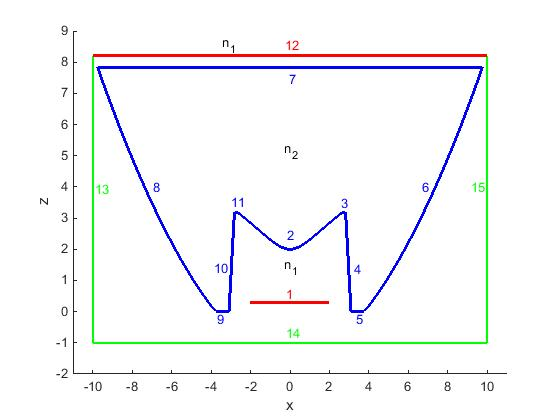
\includegraphics[width=7.7cm]{TIR}
  \end{center}
  \caption{Shape of the TIR-collimator. Each surface of the system is labeled with a number.
   The shape of the collimator is shown with a blue line.
   Three detectors depicted with green lines (surfaces $13$, $14$, and $15$) are located at the left, the right and the bottom of the optical system.
The sagitta of the lens is approximately $1.17$}
  \label{fig:tir}
\end{figure}
\\ \indent
Using PS ray tracing explained in Section \ref{sec:PS_raytracing} with around $1.9 \cdot 10^4$ rays traced, seven different paths are found. In Figure \ref{fig:sourcePS} the distribution of the rays traced at the source PS \set{S}{}{} is shown, where we depicted with the same color the rays that follow the same path. Seven different paths are found. The yellow rays follow path $\Pi_1 = (1, 2, 7, 12)$;
   the red rays follow path $\Pi_2 ~= ~(1, 10, 8, 7, 12)$; the green rays follow path $\Pi_3 = (1, 4, 6, 7, 12)$;
   the blue rays follow path $\Pi_4= (1, 11, 7, 12)$ and the magenta rays follow path $\Pi_5= (1, 3, 7, 12)$. The rays located inside the white areas correspond to rays that do not reach the target, they follow either path $\Pi_6 = (1, 10, 7, 8, 13)$ or path $\Pi_7 = (1,4,7,6,15)$ and they do not give any contribution to the target intensity.
\begin{figure}[h]
  \begin{center}
  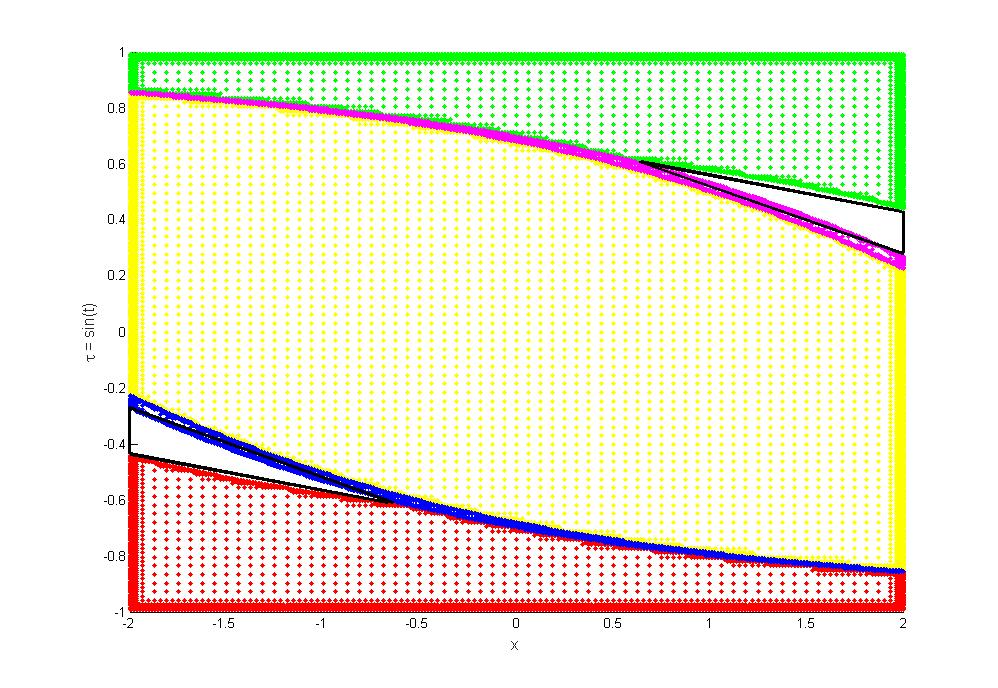
\includegraphics[width=7.7cm]{source1}
  \end{center}
  \caption{Distribution of the rays on \point{S}{}{}. Around $1.9 \cdot 10^4$ rays are traced using the triangulation refinement with parameters:
  $\varepsilon_\variabile{q}^\textrm{max} = 0.1 ,$ $ \varepsilon_{\variabile{p}}^\textrm{max} = 5\cdot 10^{-2}, $ $\varepsilon_{\variabile{q}}^\textrm{min} = 9\cdot 10^{-3}, \varepsilon_\variabile{p}^\textrm{min} = 4.5 \cdot 10^{-3}$. Rays that belong to the same region are depicted with the same color. The rays located inside the white areas do not reach the target. The boundaries of the two white regions are approximated by triangles depicted with black lines.}
  \label{fig:sourcePS}
\end{figure}
Note that, given two adjacent paths the regions $\mbox{\set{R}{$1$}{}}(\Pi)$ in \set{S}{}{} have usually a common boundary. 
Since for this system not all the rays emitted by the source arrive to the target, the target \'{e}tendue $U_{\textrm{t}}$ needs to be compared with the \'{e}tendue $U_1$ at the source given by only those rays that reach the target (the rays that follow paths $\Pi_6=(1,10,8,7,12)$ and 
$\Pi_7 = (1,4,7,6,15)$ are discarded). To this purpose $U_1$ is calculated by removing from the total area $U$ of \set{S}{}{} those areas occupied by the regions formed by the rays that hit the left and the right detector (white regions in Figure $\ref{fig:tir}$).  For the TIR colllimator in Figure \ref{fig:tir} $U = 8$. Hence, $U_1$ can be approximated by:
 \begin{equation}\label{eq:Usource}
 U_{1}\approx 8-2A_{T},
 \end{equation}
 where $A_{T}$ is the approximated area of each of the white regions in Figure $\ref{fig:tir}$ that is the area of the triangles shown in Fig. \ref{fig:sourcePS} with black lines.\\ \indent  $U_{\textrm{t}}$ is calculated several times from Equation (\ref{eq:etenduetarg}) where every time the boundaries $\partial$\set{R}{}{}$(\Pi)$ are obtained by using $\alpha$-shapes for a different value of $\alpha$. The better approximation of $\partial$\set{R}{}{}$(\Pi)$ gives the closer value of $U_{\textrm{t}}$ to the exact \'{e}tendue. 
Matching $U_1$ with all the approximation of $U_{\textrm{t}}$ we find the best value $\alpha_c$ of $\alpha$ that approximates $\partial$\set{R}{}{}$(\Pi)$ and, therefore, $U_{\textrm{t}}$. \\ \indent In Figure \ref{fig:etendueTS} we represent the approximated value of the source \'{e}tendue $U_1\approx 7.68$ with the dotted red line obtained from Equation (\ref{eq:Usource}). Different approximations of the target \'{e}tendue $U_{\textrm{t}}$ are calculated using Equation (\ref{eq:etenduetarg1}) where every time the boundaries $\partial$\set{R}{}{}$(\Pi)$ are found using $\alpha$-shapes with a different value of $\alpha$. In Figure \ref{fig:etendueTS} we show how the \'{e}tendue change by increasing the value of $\alpha$. Doing $10$ different $\alpha$ test we compute the '{e}tendue behavior which is depicted with the blue line in Figure \ref{fig:etendueTS}. This graph    
shows that using PS ray tracing with $1.9\cdot 10^4$ rays, the best approximation of the boundaries $\partial$\set{R}{}{}$(\Pi)$ is given considering $\alpha = \alpha_c = 0.041$ in the $\alpha$-shapes procedure.
 \begin{figure}[h]
  \begin{center}
  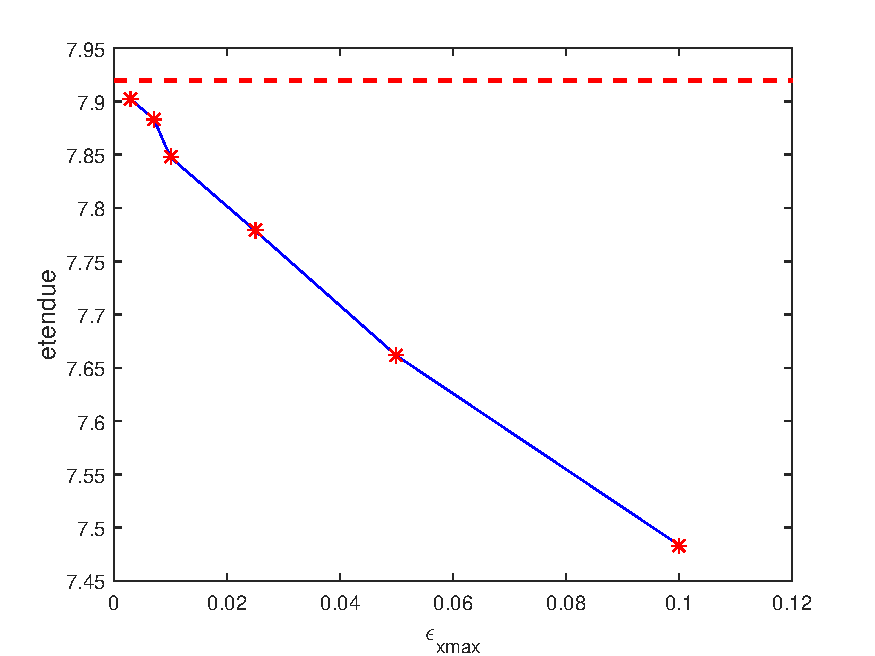
\includegraphics[width=7.7cm]{etendue}
  \end{center}
  \caption{\footnotesize{The source and the target \'{e}tendue are depicted with the dotted red line and the blue line, respectively.
  $U_\textrm{t}$ is computed for a range of values for $\alpha$. $U_1 \approx 7.68$
   The green dot indicates the value of $\alpha_c = 0.041$ which gives the best approximation of the boundaries $\partial$\set{R}{}{}$(\Pi)$ at the target.
   Around $1.9 \cdot 10^4$ rays have been traced in PS.
  }}
  \label{fig:etendueTS}
\end{figure}
Applying $\alpha$-shapes with $\alpha=\alpha_c$, a good approximation of $\partial$\set{R}{}{}$(\Pi)$ is found. In Fugure \ref{fig:targetPS} we show the boundaries 
$\partial$\set{R}{}{}$(\Pi)$ in target PS \set{T}{}{} with $\alpha_c=0.041$ and tracing $1.9\cdot10^4$ rays.
  \begin{figure}[h]
  \begin{center}
  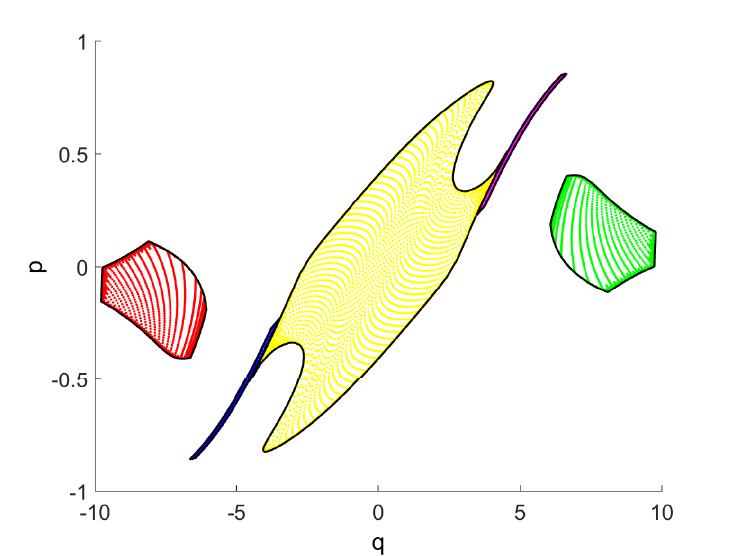
\includegraphics[width=7.7cm]{target_alpha_shapes.png}
  \end{center}
  \caption{\footnotesize{Target PS representation of a set of $1.9 \cdot 10^4$ rays.
  Rays that follow the same path are depicted with the same color. The choice of the colors for each path is the same as in Figure $\ref{fig:sourcePS}$. The boundaries $\partial$\set{R}{}{}$(\Pi)$ are computed through the $\alpha$-shapes method with $\alpha = \alpha_c = 0.041$.}}
  \label{fig:targetPS}
\end{figure}
Once the boundaries are computed, the target intensity $I_{\textrm{PS}}(\variabile{p})$ for every $\variabile{p}\in[-1,1]$ is obtained from Equation (\ref{eta2}). \\ \indent
To validate our method we compare the PS intensity with the MC intensity. 
To this purpose a partitioning $P_2:-1=\variabile{p}_{0}<\variabile{p}_1<\cdots<\variabile{p}_{\nbin}=1$ of the interval $[-1,1]$ into $\nbin=100$ bins is considered. 
The averaged and normalized PS intensity $\hat{I}_{\textrm{PS}}$ is calculated for every 
$\big(\variabile{p}^{\variabile{h}+1/2} = \frac{1}{2}(\variabile{p}^{\variabile{h}+1}, \variabile{p}^{\variabile{h}})\big)_{\variabile{h}=0, \cdots, \nbin-1}$ dividing the PS averaged intensity by the total \'{e}tendue:
\begin{equation}\label{eq:normalized_PS_intensity}
\hat{I}_{\textrm{PS}}(\variabile{p}^{\variabile{h}+1/2}) = \frac{1}{U_{\textrm{t}}}\int_{\variabile{p}_{\variabile{h}}}^{\variabile{p}_{\variabile{h}+1}} I_{\textrm{PS}}(\variabile{p})\textrm{d}\variabile{p}
\end{equation}
The averaged and normalized MC intensity $\big(\hat{I}_{\textrm{MC}}(\variabile{p}^{\variabile{h}+1/2})\big)_{\variabile{h} = 0, \cdots, \nbin-1}$ intensity is given by
\begin{equation}\label{eq:normalized_MC_intensity}
\hat{I}_{\textrm{MC}}(\variabile{p}^{\variabile{h}+1/2}) = \frac{\nrays[\variabile{p}^{\variabile{h}-1},\variabile{p}^{\variabile{h}})}{\nrays [-1,1)} 
\qquad \mbox{ for } \variabile{p}\in[\variabile{p}^{\variabile{h}-1}, \variabile{p}^{\variabile{h}}).
\end{equation} 
Both the approximate intensities $\hat{I}_{\textrm{A}} (\textrm{A} = \textrm{PS}, \textrm{MC})$ are compared with an intensity $\hat{I}_{\textrm{ref}}$ taken as a reference. For some optical systems, there is an explicit solution for the target intensity but this is not the case of the TIR-collimator.
Therefore, a MC simulation with $1.7 \cdot 10^8$ rays is run to obtain the averaged normalized intensity $\hat{I}_{\mbox{ref}}$ which is used as reference.
The intensity profile $\hat{I}_{\textrm{PS}}
$ obtained using PS ray tracing with $66\,855$ rays and $\alpha= \alpha_c = 0.02$ is depicted in Fig. \ref{fig:intensityMCPS} with a red line.
$\hat{I}_{\textrm{PS}}$ is hardly distinguishable from $\hat{I}_{\mbox{ref}}$ (dashed and blue line in Figure $\ref{fig:intensityMCPS}$).\\ \indent
  \begin{figure}[h]
    \centering
    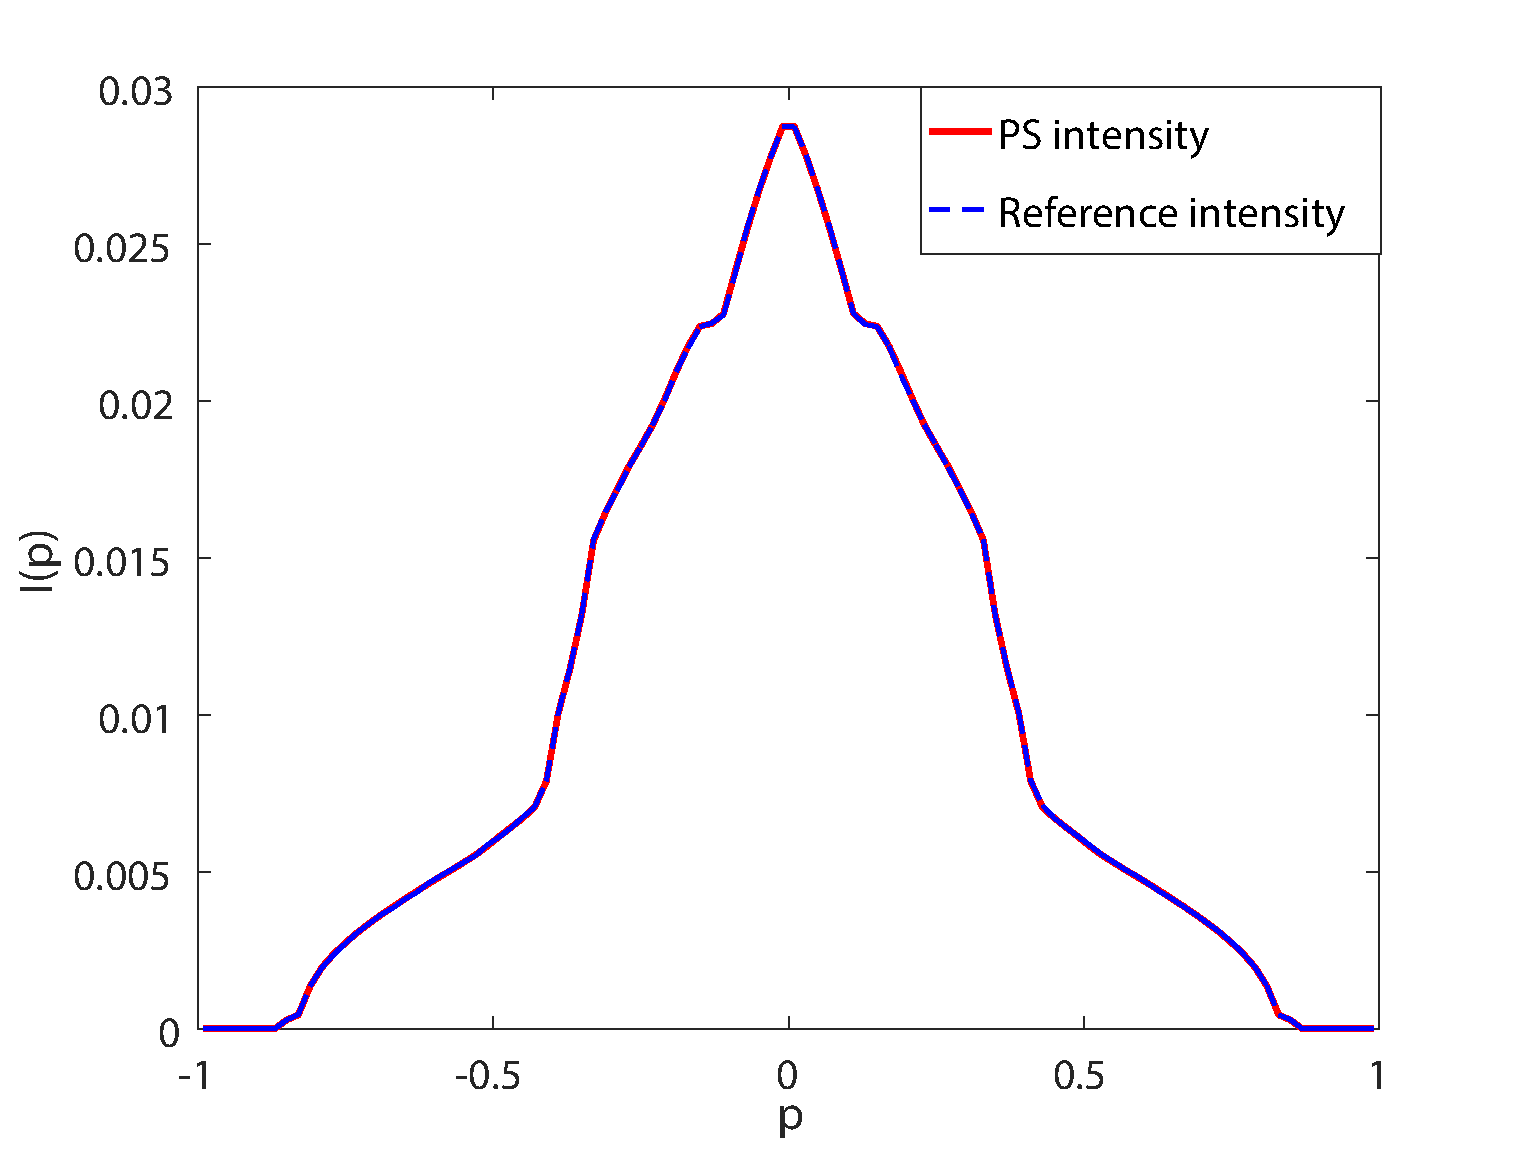
\includegraphics[width=7.7 cm]{intensity_alpha_shapes}
\caption{The red line shows the PS intensity at the target of the TIR-collimator. The exact intensity is depicted with the dotted blue line.
The exact intensity is computed using the MC method for a set of $15$ millions of rays. For the PS intensity a set of $6.6\cdot 10^4$
rays is considered and $\alpha_c = 0.02$ is chosen to compute the boundaries $\partial$\set{R}{}{}$(\Pi)$. The approximate intensity can hardly be distinguished from the reference intensity.}
  \label{fig:intensityMCPS}
\end{figure}
Finally, we calculate the error between $\hat{I}_{\textrm{A}}$ and $\hat{I}_{\textrm{ref}}$, defined as:
\begin{equation}\label{eq:error}
\mbox{error} = \frac{\sum_{\variabile{h}= 1}^{\nbin}| \hat{I}_{A}(\variabile{p}^{\variabile{h}}) - \hat{I}_{\mbox{ref}}(\variabile{p}^{\variabile{h}})|}{\nbin}.
\end{equation}
The MC and PS intensities are calculated several times increasing the number of rays to improve the accuracy.
Tables \ref{tab:table} and \ref{tab:table2} describe how the number of rays traced affects the error. 
In Table \ref{tab:table} a correlation between $\alpha_c$ and the number of rays is shown.
%determined by the values of $\varepsilon^{\textrm{min}}_\variabile{p}$, $\varepsilon^{\textrm{min}}_{\variabile{q}}$, 
%$\varepsilon^{\textrm{max}}_{\variabile{p}}$ and $\varepsilon^{\textrm{max}}_{\variabile{q}}$. 
Note that increasing the number of rays the value of $\alpha_c$ and the corresponding error decrease. 
\begin{table}[htbp] \label{tab:table}
\centering
\caption{\bf Error values of the PS intensity}
\begin{tabular}{lllllll}

 \hline  Number \\ of rays\;  & $\varepsilon^{\textrm{max}}_{\variabile{q}} $  & $\varepsilon^{\textrm{min}}_{\variabile{q}} $   \;     & $\varepsilon^{\textrm{max}}_{\variabile{p}}$\;
  & $\varepsilon^{\textrm{min}}_\variabile{p}$\; & $\alpha_c$  & PS error \\
  \hline 
 $3\,363$ & $0.9$  & $0.1$  & $0.50$  & $0.025$ & $0.119$ & $1.20\cdot10^{-3}$ \\
$6\,949$  & $0.5$  & $0.050$  & $0.25$  & $0.020$ & $0.098$ & $2.50\cdot 10^{-4}$  \\
$15\,870$  & $0.4$  & $0.025$  & $0.02$  & $0.001$ & $0.050$ & $5.49\cdot 10^{-5}$ \\
 $37\,455$  & $0.2$  & $0.020$  & $0.10$ & $0.005$ & $0.037$ & $2.00\cdot 10^{-5}$ \\
 $66\,855$ & $0.1$  & $0.009$  & $0.05$  & $0.004$ & $0.020$ & $1.00\cdot 10^{-5}$ \\
 \hline
 \end{tabular}
 \label{tab:table}
 \end{table}
\\ \indent In Table \ref{tab:table2} the numerical results of MC ray tracing are reported.
Increasing the number of rays traced in MC ray tracing, the error gradually decreases.
\begin{table}[htbp]
\centering
\caption{\bf Error values of the MC intensity}
\begin{tabular}{ll} \hline   Number of rays\; & MC error\\ \hline $972$  & $2.10\cdot10^{-3}$ \\
$9\,714$  & $6.69\cdot 10^{-4}$  \\ $97\,103$  & $2.08\cdot 10^{-4}$ \\ $971\,627$  & $7.00\cdot 10^{-5}$ \\ $9\,716\,519$  & $2.00\cdot 10^{-5}$ \\
 \hline
 \end{tabular}
 \label{tab:table2}
 \end{table}
\noindent In Figure $\ref{fig:error}$, the results listed in Table $\ref{tab:table}$ and Table $\ref{tab:table2}$ are shown. The red line depicts the convergence of the PS error and the blue line indicates the MC error.
\begin{figure}[h!]
  \begin{center}
  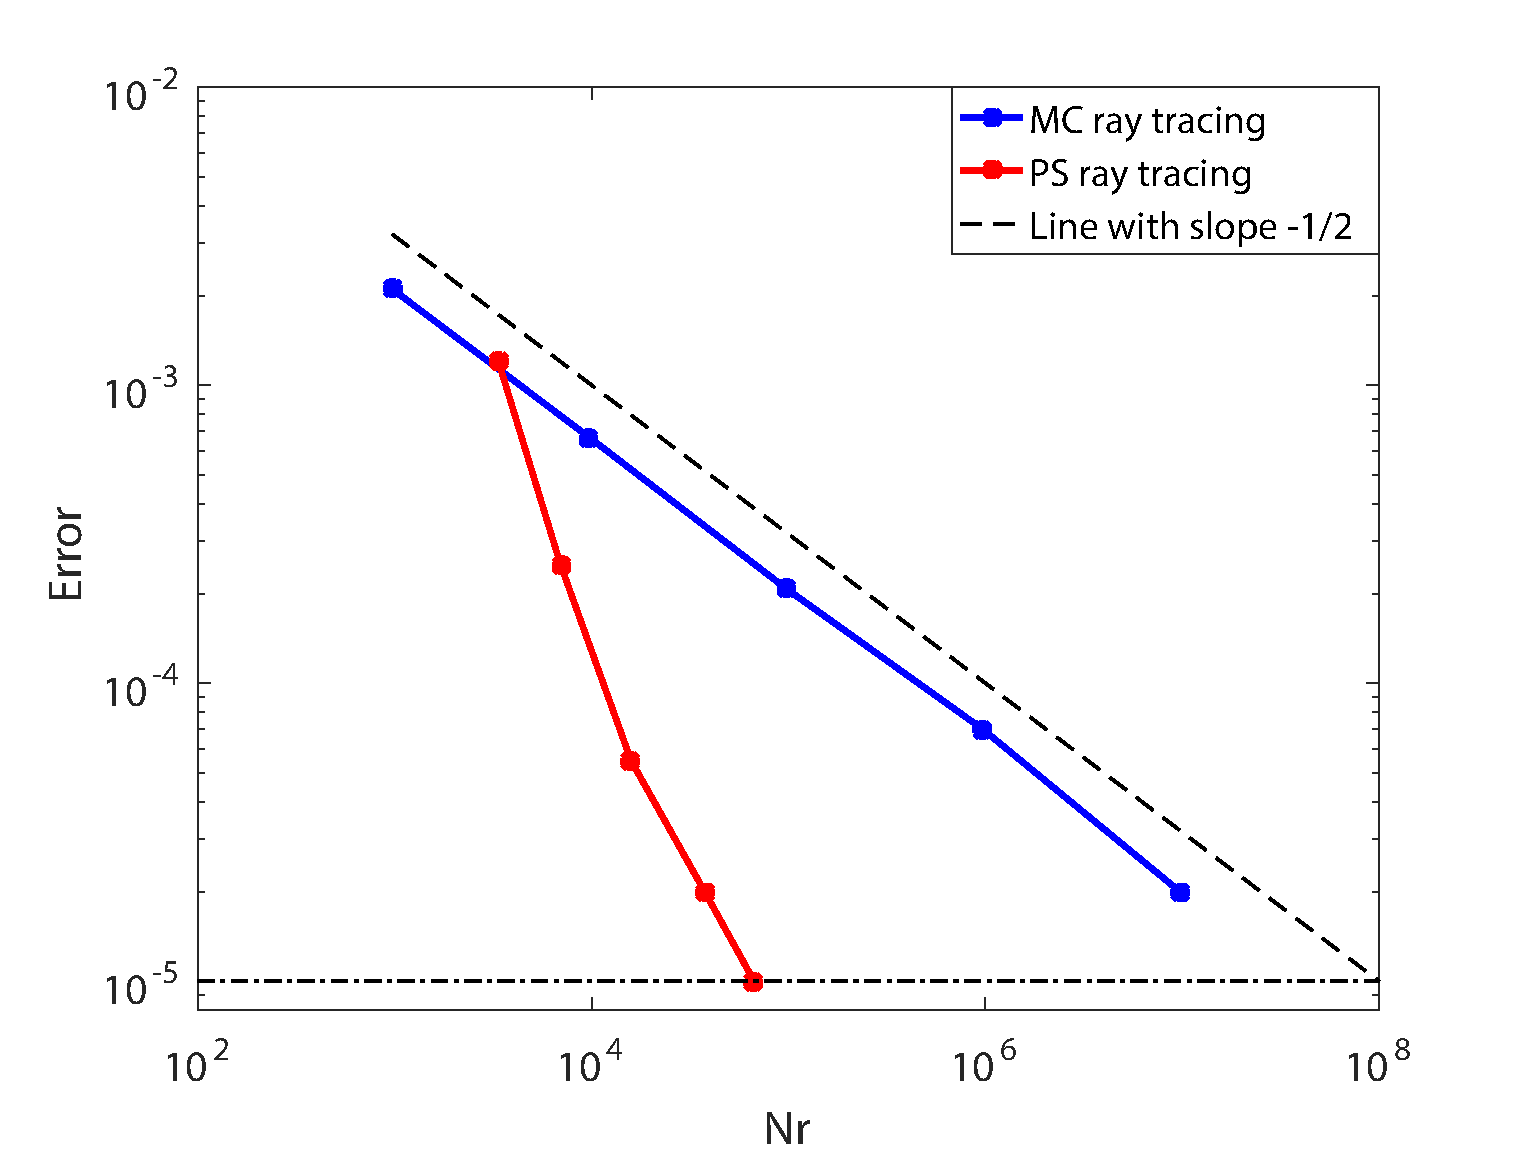
\includegraphics[width=7.7cm]{error_alpha_shapes1}
  \end{center}
  \caption{\footnotesize{ The red line depicts the error between the PS intensity and the reference intensity.
 The blue line shows the error between the MC intensity and the reference intensity.
  The dashed line represents a straight line with the slope equal to $-\frac{1}{2}$.
  The horizontal dotted line shows that an error equal to $2.00 \cdot  10^{-5}$ can be obtained tracing at least $10^2$ times fewer rays in phase space.}}
  \label{fig:error}
\end{figure}
Note from Figure \ref{fig:error} that the error for the MC method decreases as $\frac{1}{\sqrt{Nr}}$, while for the PS simulation the speed of convergence is much higher.\\ \indent
We need to emphasize that the PS ray tracing convergence may change according to the design of the optical system.
This is because the approximation of the boundaries in PS depends on the accuracy of the $\alpha$-shapes method.
The $\alpha$-shapes is unable to detect properly the boundaries of regions with a sharp turn if not enough points are given
\cite{teichmann1998surface}. Indeed, on the one hand a low density requires a big values of $\alpha$ to accept the triangles in a region, on the other hand,
 choosing $\alpha$ big, the shape of the region could be destroyed (some rays inside the regions could be taken into account).
 \begin{figure}[h]
\centering
  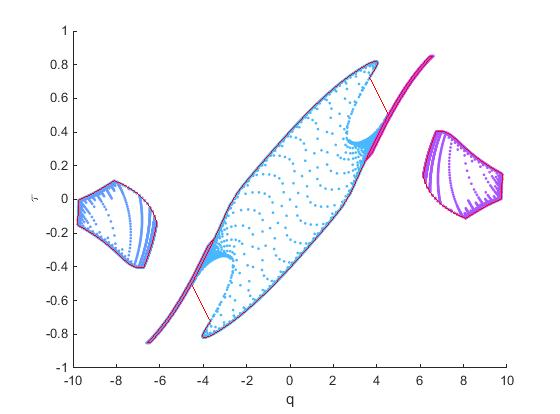
\includegraphics[width=7.7cm]{Tir1}
    \caption{Target PS for the TIR-collimator depicted in
    Figure \ref{fig:tir}. The red line depicts the best approximations of $\partial$\set{R}{}{}$(\Pi)$ for $3363$ rays with $\alpha_c = 0.119$.
    The cyan region in the middle of the target PS is formed by rays that hit the lens, it is hard to approximate that region when there is a small number of rays inside it.}
     \label{fig:Tir1}
  \end{figure}
Figure $\ref{fig:Tir1}$ clarifies this concept showing that the region formed by rays that hit the lens is hard to approximate when there is a small number of rays inside the region. Consequently either a region bigger than the area covered by the rays is considered or some triangles which are not part of the boundaries are considered in the triangulation. This results in an inaccurate calculation of the intensity (either too high or to low). To obtain a good approximation of the boundaries of these kind of patches more rays have to be traced. Therefore, the error in the approximate intensity is rather big for few rays (compared to MC error) and it decreases very fast increasing the number of rays (see Table
 \ref{tab:table} and Figure \ref{fig:error}).
 \\
 \indent To show how the error plot changes according to the regularity of the shape of the regions $\partial$\set{R}{}{}$(\Pi)$, we consider another example of TIR-collimator.
 Figure $\ref{fig:Tir1}$ shows that the hardest region to approximate is given by those rays that follow the path $\Pi_1 ~=~ (1,2,7,12)$.
 We now consider the TIR-collimator shown in Figure $\ref{fig:analyticlens}$. The difference with the previous optical system considered is that the lens is flatter and the target is located at a closer distance from the top.
Figure $\ref{fig:Tir2}$ shows that a flatter lens removes one of the two spikes of the region formed by the rays that hit the lens.
Moreover a target located very close to the top makes the shape of that region less stretched along the $\variabile{q}$-axis.
Therefore, it is expected that $\alpha$-shapes method performs well, even for a small number of rays.
\begin{figure}[h]
  \begin{center}
  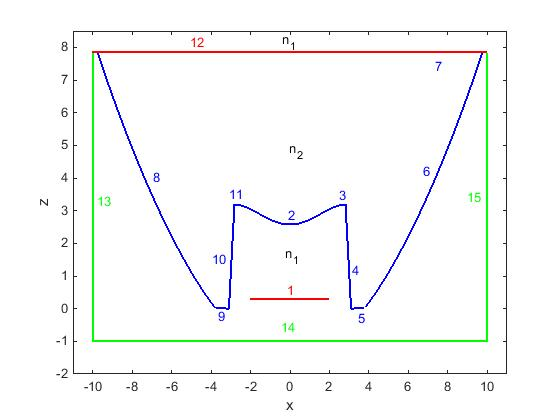
\includegraphics[width=6.5cm]{tir_analytic2}
   \end{center}
    \caption{\footnotesize{Shape of the TIR-collimator. Each surface of the system is labeled with a number.
       The source $\mathcal{S}= [-2,2]$ (surface number $1$) is located at a height $\variabile{z}_1 = 0.3$ from the $x$-axis.
       The target $\mathcal{T}= [-9.7, 9.7]$ (surface $12$) is parallel to the source and is located at a height $ \variabile{z}= 7.85$.
       The shape of the collimator is shown as a blue line.
       Three detectors depicted with green lines (surfaces $13$, $14$, and $15$) are located at the left, the right and the bottom of the optical system.
       $n_1 = 1$ is the refraction index of the medium (air) where the source and the target are located, and
       $n_2 = 1.5 $ the refraction index of the medium (glass) inside the optical system. The sagitta of the lens is equal to $0.6$}}
 \label{fig:analyticlens}
\end{figure}
 \begin{figure}[h]
  \begin{center}
       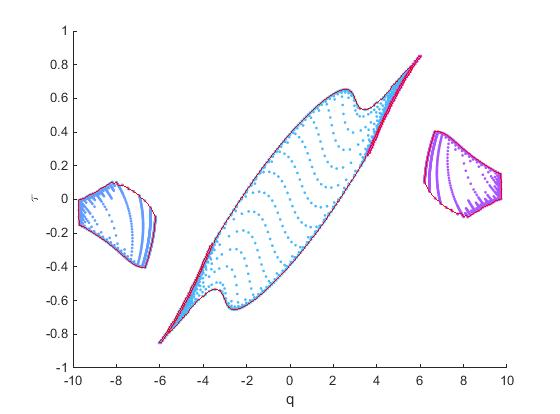
\includegraphics[width=7.7cm]{Tir2}
   \end{center}
        \caption{Target phase space for the TIR-collimator depicted in
        Figure \ref{fig:analyticlens}. The red line depicts the best approximation of $\partial$\set{R}{}{}$(\Pi)$ for $3363$ rays. The value of $\alpha$ is $0.06$.
        The $\alpha$-shapes method gives an accurate approximation of the boundaries.}
  \label{fig:Tir2}
\end{figure}
 PS and MC ray tracing are implemented for the TIR-collimator in Figure \ref{fig:Tir2}. The approximated intensities $\hat{I}_{\textrm{A}}$ $(\textrm{A} = \textrm{PS}, \textrm{MC})$ are compared with the reference intensity $\hat{I}_{\textrm{ref}}$ (MC ray tracing with $10^7$ rays). The error between $\hat{I}_{\textrm{A}}$ and $\hat{I}_{\textrm{ref}}$ as a function of the number of rays is obtained from Equation (\ref{eq:error}). The convergence of PS and MC ray tracing is shown in Figure \ref{fig:error2}. 
PS error is depicted with the red line and, MC error is depicted with the blue line. Still big 
\begin{figure}[h!]
 \begin{center}
   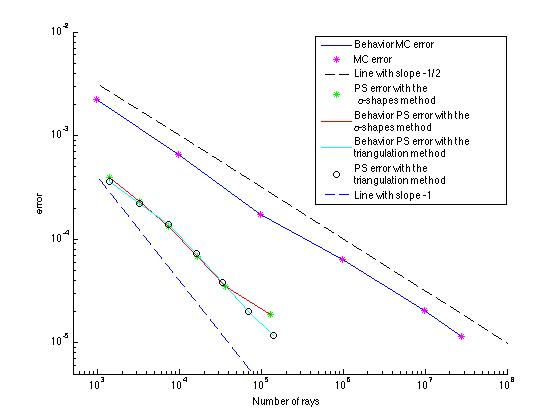
\includegraphics[width=7.7cm]{error_plot}
    \end{center}
     \caption{\footnotesize{ The red line depicts the error using the $\alpha$-shapes method to compute the boundaries. The cyan line depicts the error using the triangulation refinement to compute the boundaries.
     The blue line shows the error between the Monte Carlo intensity and the exact intensity.
     The dashed black line represents a straight line with slope $-\frac{1}{2}$.
   The dashed blue line represents a straight line with slope $-1$.}}
 \label{fig:error2}
\end{figure}
\section{Conclusion}
The aim of this chapter was to detect the boundaries of the regions formed by the rays traced using the PS ray tracing explained in Chapter \ref{chap:PS}.\\
\indent First, we reported some theory about $\alpha$-shapes methods which are common used in order to approximate the shape formed by a point cloud. 
These methods depends on a parameter $\alpha$ that in most cases can be determined only by several simulations. 
Using \'{e}tendue conservation, we developed an approach to detect the value of $\alpha$ that better approximates the boundaries in target PS. 
We applied $\alpha$-shapes to two different kinds of TIR-collimators. The target PS intensity was computed for both the systems several times increasing every time the number of rays traced. Finally, the corresponding errors between the intensities found and a reference intensity was calculated. We observed that PS ray tracing leads to trace far less rays compared to MC ray tracing. Numerical results show that using PS ray tracing the desired accuracy can be achieved reducing the number of rays traced by a factor $2$ for both the optical systems analyzed.\\ \indent 
However, the error convergence for PS ray tracing strongly depends on the design of the optical system (shapes of the region in target PS). Indeed, the intensity accuracy is related to the precision of the $\alpha$-shape, that is, to the choice of the parameter's value of $\alpha$. For more complicated shapes in PS, more rays need to be traced for a good boundaries reconstruction.\\ \indent
In order to remove the dependence of PS ray tracing from the parameter $\alpha$, we construct another procedure to detect the boundaries of the regions in target PS. 
The new technique is based only on the triangulation refinement explained in Section \ref{sec:PS_raytracing}. The details are explained in the next chapter and numerical results for several optical systems are reported. 











































